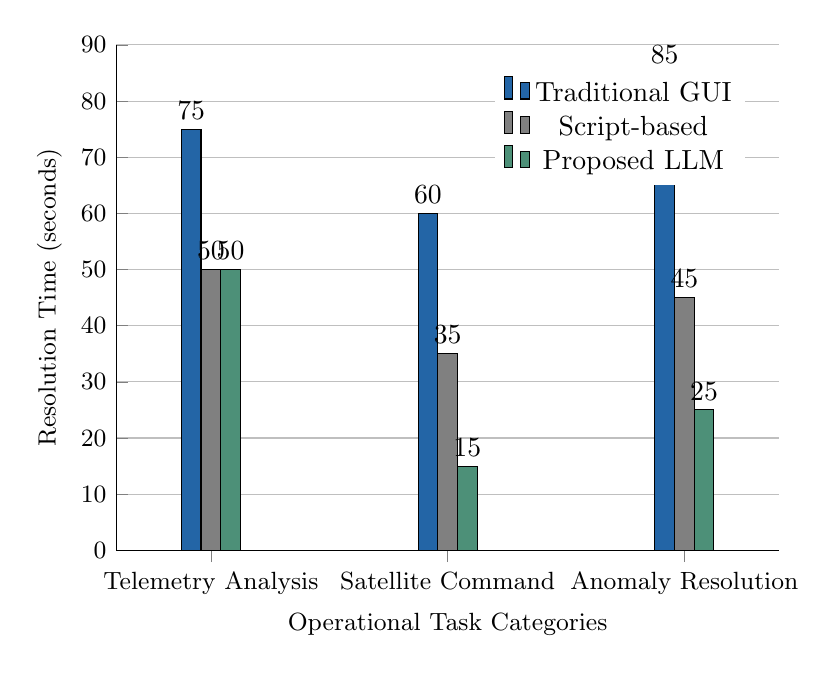
\begin{tikzpicture}
% === PARÁMETROS ===
\definecolor{colorGUI}{HTML}{2365A6}
\definecolor{colorScript}{HTML}{808080}
\definecolor{colorLLM}{HTML}{4D9078}

\pgfplotsset{
    estiloBarra/.style={
        ybar,
        bar width=0.25cm,
        nodes near coords,
        nodes near coords align={vertical},
    }
}

% === ESTRUCTURA PRINCIPAL ===
\begin{axis}[
    width=10cm, height=8cm,
    ybar=0pt, % Espaciado entre grupos
    enlarge x limits=0.2,
    symbolic x coords={Telemetry Analysis, Satellite Command, Anomaly Resolution},
    xtick=data,
    ylabel={Resolution Time (seconds)},
    xlabel={Operational Task Categories},
    ymin=0, ymax=90,
    ytick={0,10,...,90},
    ymajorgrids=true,
    grid style={gray!50},
    axis lines*=left,
    legend style={at={(0.95,0.95)}, anchor=north east, draw=none},
    tick label style={font=\small},
    label style={font=\small}
]

% === DATOS ===
\addplot[fill=colorGUI, estiloBarra] coordinates {
    (Telemetry Analysis, 75) (Satellite Command, 60) (Anomaly Resolution, 85)
};
\addlegendentry{Traditional GUI}

\addplot[fill=colorScript, estiloBarra] coordinates {
    (Telemetry Analysis, 50) (Satellite Command, 35) (Anomaly Resolution, 45)
};
\addlegendentry{Script-based}

\addplot[fill=colorLLM, estiloBarra] coordinates {
    (Telemetry Analysis, 50) (Satellite Command, 15) (Anomaly Resolution, 25)
};
\addlegendentry{Proposed LLM}

\end{axis}
\end{tikzpicture}